\documentclass[14pt,aspectratio=169]{beamer}
\setbeamertemplate{caption}[numbered]
\setbeamertemplate{caption label separator}{:}
\setbeamercolor{caption name}{fg=normal text.fg}
\usepackage{amssymb,amsmath}
\usepackage{ifxetex,ifluatex}
\usepackage{fixltx2e} % provides \textsubscript
\usepackage{lmodern}
\ifxetex
  \usepackage{fontspec,xltxtra,xunicode}
  \defaultfontfeatures{Mapping=tex-text,Scale=MatchLowercase}
  \newcommand{\euro}{€}
\else
  \ifluatex
    \usepackage{fontspec}
    \defaultfontfeatures{Mapping=tex-text,Scale=MatchLowercase}
    \newcommand{\euro}{€}
  \else
    \usepackage[T1]{fontenc}
    \usepackage[utf8]{inputenc}
      \fi
\fi
% use upquote if available, for straight quotes in verbatim environments
\IfFileExists{upquote.sty}{\usepackage{upquote}}{}
% use microtype if available
\IfFileExists{microtype.sty}{\usepackage{microtype}}{}
\PassOptionsToPackage{hyphens}{url}
\usepackage{hyperref}
\usepackage{ulem}

% Comment these out if you don't want a slide with just the
% part/section/subsection/subsubsection title:
\AtBeginPart{
  \let\insertpartnumber\relax
  \let\partname\relax
  \frame{\partpage}
}
\AtBeginSection{
  \let\insertsectionnumber\relax
  \let\sectionname\relax
  \begin{frame}[plain]
    \tableofcontents[currentsection]
  \end{frame}
}
\AtBeginSubsection{
  \let\insertsubsectionnumber\relax
  \let\subsectionname\relax
  \frame{\subsectionpage}
}

\setlength{\parindent}{0pt}
\setlength{\parskip}{6pt plus 2pt minus 1pt}
\setlength{\emergencystretch}{3em}  % prevent overfull lines
\setcounter{secnumdepth}{0}
% Thanks Richard Darst on how to get a nice Beamer theme.
% See http://rkd.zgib.net/wiki/DebianBeamerThemes

\usepackage{multicol}
\usepackage[absolute,overlay]{textpos}
\usepackage{tikz}
\usepackage{ctable}
\usetikzlibrary{positioning}

\usebackgroundtemplate{
\includegraphics[width=\paperwidth]{images/swirl-lightest.pdf}}
\newif\ifplacelogo
\placelogotrue
\logo{\ifplacelogo
\includegraphics[viewport=274 335 360 440,width=1cm]{images/openlogo-nd.pdf}\fi}

\definecolor{debianred}{rgb}{.780,.000,.211} % 199,0,54
\definecolor{debianblue}{rgb}{0,.208,.780} % 0,53,199
\definecolor{debianlightbackgroundblue}{rgb}{.941,.941,.957} % 240,240,244
\definecolor{debianbackgroundblue}{rgb}{.776,.784,.878} % 198,200,224

\usetheme{Boadilla}
\setbeamertemplate{navigation symbols}{}

\usecolortheme[named=debianbackgroundblue]{structure}
\setbeamercolor{normal text}{fg=black}
\setbeamercolor{titlelike}{fg=debianblue}
\setbeamercolor{sidebar}{fg=debianred,bg=debianbackgroundblue}

\setbeamercolor{palette sidebar primary}{fg=debianred}
\setbeamercolor{palette sidebar secondary}{fg=debianred}
\setbeamercolor{palette sidebar tertiary}{fg=debianred}
\setbeamercolor{palette sidebar quaternary}{fg=debianred}

\setbeamercolor{section in toc}{fg=debianred}
\setbeamercolor{subsection in toc}{parent=debianred}

\setbeamercolor{item}{fg=debianred}

\setbeamercolor{block title}{fg=debianblue}

\title[Reproducible builds everywhere]{Reproducible
builds everywhere \\ eg. in Debian, OpenWrt and LEDE}
\subtitle{Bit by bit identical binaries \\
from a given source}
\author[h01ger and lynxis]{%
   \texorpdfstring{
            \centering
            Alexander 'lynxis' Couzens\\
            Holger 'h01ger' Levsen
   }{h01ger and lynxis}}
\date[OpenWrt Summit, Berlin]{%
 OpenWrt Summit in Berlin, Germany\\
 \small{2016-10-13}}

\begin{document}

\begin{frame}[plain]
 \titlepage
\end{frame}

\begin{frame}
 \frametitle{about h01ger}

 \begin{itemize}
  \item \small{\texttt{B8BF 5413 7B09 D35C F026  FE9D 091A B856 069A AA1C}}
  \item Debian user since 1995
  \item Debian contributor since 2001
  \item OpenWrt user since 2006
  \item Debian developer since 2007
  \item \underline{DebConf organizer},
  founded the DebConf video team
   \begin{itemize}
    \item \texttt{http://video.debian.net}
   \end{itemize}
 \item \underline{Debian-Edu} (Debian for education)
  \item Debian QA (quality assurance)
  \begin{itemize}
   \item \texttt{https://piuparts.debian.org}
   \item \texttt{https://jenkins.debian.net} (~1200 jobs continously testing Debian)
  \end{itemize}
  \item \underline{Debian LTS} (Long Term Support)
  \item Debian Reproducible builds team member
  \begin{itemize}
   \item since April 2015 funded by the Linux Foundation
 \end{itemize}
 \end{itemize}
\end{frame}

\begin{frame}
 \frametitle{about lynxis}

 \begin{itemize}
  \item Debian user since 2003
  \item OpenWrt user since 2006
  \item LEDE founding member
  \item coreboot hacker
  \item tests.reproducible-builds.org contributor
  \item ex-GSoC student
  \item CCC member
 \end{itemize}
\end{frame}


\begin{frame}
 \frametitle{Debian reproducible builds team}
 \begin{center}
  \begin{columns}
   \small
   \column{.30\linewidth}
    {akira} \\
    {Andrew Ayer} \\
    {Asheesh Laroia} \\
    {Chris Lamb} \\
    {Chris West} \\
    {Christoph Berg} \\
    {Daniel Kahn Gillmor} \\
    David Suarez \\
    {Dhole} \\
    Drew Fisher \\
    Esa Peuha \\
    {Guillem Jover} \\
   \column{.30\linewidth}
    Hans-Christoph Steiner \\
    {Helmut Grohne} \\
    \only<1>{Holger Levsen}\only<2>{{\color{debianred} Holger Levsen}} \\
    {Jelmer Vernooij} \\
    {josch} \\
    Juan Picca \\
    {Lunar} \\
    Mathieu Bridon \\
    {Mattia Rizzolo} \\
    Nicolas Boulenguez \\
    {Niels Thykier} \\
    Niko Tyni \\
   \column{.30\linewidth}
    {Paul Wise} \\
    Peter De Wachter \\
    Philip Rinn \\
    {Reiner Herrmann} \\
    {Stefano Rivera} \\
    {Stéphane Glondu} \\
    {Steven Chamberlain} \\
    Tom Fitzhenry \\
    Valentin Lorentz \\
    {Wookey} \\
    {Ximin Luo} \\
  \end{columns}
 \end{center}
\end{frame}

\begin{frame}
 \frametitle{jenkins.debian.net.git contributors}
 \begin{center}
  \begin{columns}
   \small
   \column{.46\linewidth}
    {akira} \\
    \only<1>{Alexander Couzens}\only<2>{{\color{debianred} Alexander Couzens}} \\
    \only<1>{Levente 'anthraxx' Polyak}\only<2>{{\color{debianred} Levente 'anthraxx' Polyak}} \\
    {Antonio Terceiro} \\
    {Axel Beckert} \\
    \only<1>{Bryan Newbold}\only<2>{{\color{debianred} Bryan Newbold}} \\
    {Chris Lamb} \\
    {Daniel Kahn Gillmor} \\
    {Gabriele Giacone} \\
    \only<1>{Hans-Christoph Steiner}\only<2>{{\color{debianred} Hans-Christoph Steiner}} \\
    Helmut Grohne \\
    \only<1>{Holger Levsen}\only<2>{{\color{debianred} Holger Levsen}} \\
    \only<1>{HW42}\only<2>{{\color{debianred} HW42}} \\
    {James McCoy} \\
    {Joachim Breitner} \\
   \column{.46\linewidth}
    {Johannes 'josch' Schauer} \\
    {Jérémy Bobbio} \\
    {Mattia Rizzolo} \\
    {Niels Thykier} \\
    {Paul Wise} \\
    {Petter Reinholdtsen} \\
    {Philip Hands} \\
    \only<1>{Reiner Herrmann}\only<2>{{\color{debianred} Reiner Herrmann}} \\
    {Samuel Thibault} \\
    {Steven Chamberlain} \\
    {Tails developers} \\
    {Ulrike Uhlig} \\
    {Wolfgang Schweer} \\
    {Wouter Verhelst} \\
  \end{columns}
 \end{center}
\end{frame}


\begin{frame}
 \frametitle{Who are you?}
 \begin{itemize}
  \item<2-4> Seen a talk about reproducible builds?
  \item<3-4> Contributed to the efford?
  \item<3-4> Uses Debian or a Debian based system?
 \end{itemize}
\end{frame}


\section{Motivation}

\begin{frame}
 \frametitle{The problem}

 \begin{center}
  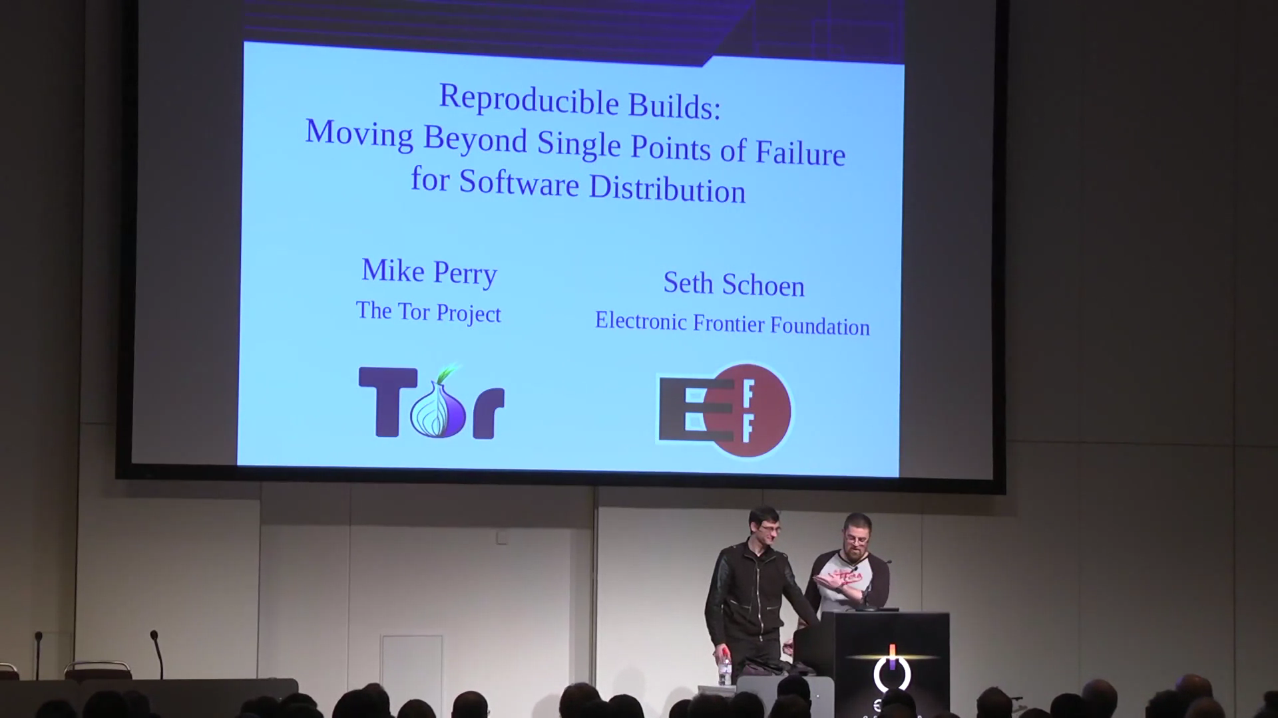
\includegraphics[width=0.7\textwidth]{images/31c3.png}

  Available on \url{media.ccc.de}, 31c3
 \end{center}
\end{frame}

\begin{frame}[fragile]
 \frametitle{A few examples from that 31c3 talk}
 \begin{itemize}
  \item CVE-2002-0083: remote root exploit in \texttt{sshd}, a single bit difference in the binary
  \item<2-5> 31c3 talk had a live demo with a kernel module modifying source code in memory only
  \item<3-5> financial incentives to crack developer machines or a projects
  build infrastructure…
  \item<4-5> {how can you be sure what's running on your machine or on a build
  daemon network? Do you ever leave your} \only<4>{USB3 ports alone?}\only<5>{computers alone?}
 \end{itemize}
\end{frame}

\begin{frame}[fragile]
 \frametitle{Another example from real life}

 At a CIA conference in 2012:
 \begin{center}
  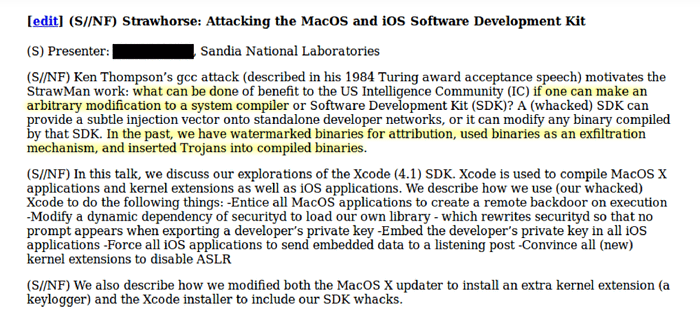
\includegraphics[width=0.8\textwidth]{images/strawhorse.png}

  {\footnotesize
  \url{firstlook.org/theintercept/2015/03/10/ispy-cia-campaign-steal-apples-secrets/}
  }
 \end{center}
\end{frame}


\begin{frame}
 \frametitle{The solution}

 \begin{center}
 \Large{
 Promise that anyone can always generate
 identical binary packages
 from a given source}
\end{center}
\end{frame}


\begin{frame}
 \frametitle{The solution}

 \begin{center}
 We call this:

 \Huge{ “Reproducible builds” }
 \end{center}
\end{frame}

\begin{frame}
 \frametitle{Demo}
 \begin{itemize}
 \item<2-3> Build a package 5 times, get 5 .debs with different checksums
 \item<3> Build a package 5 times, get 5 .debs with the same checksum
 \end{itemize}
% show this once running in plain sid,
% and then in sid with our modified toolchain.
%
% prepare demo:
% mkdir demo ; cd demo ; apt-get source giftrans
%
% do demo:
% PTH=$(mktemp -d); OPTH=$PWD; P=giftrans; cp ${P}_* $PTH/; cd $PTH ;
%   dpkg-source -x ${P}*.dsc ; for X in 1 2 3 4 5 ; do (cd ${P}-*/;
%   dpkg-buildpackage -b -uc -us); mkdir -p .$X ; cp $P_*.deb .$X; done ; rm
%   *.deb ; echo; sha1sum *dsc *z .*/*.deb | grep -v giftrans-dbgsym ; cd - ;
% rm -r $PTH
\end{frame}

\begin{frame}[plain]
\begin{center}
 \Huge{This should become the \textbf{norm}.}

 \visible<2>{\small{ We want to change the meaning of "free software":

  it's only free software if it's reproducible!}}
\end{center}
\end{frame}

\begin{frame}[fragile]
 \frametitle{More benefits than "just" security…}
 \begin{itemize}
  \item smaller deltas, thus faster updates possible
  \item in Debian: lots of QA benefits
  \item Google does reproducible builds, to save money
  \item …
 \end{itemize}
\end{frame}



\section{Common ressources}

\begin{frame}
 \frametitle{reproducible-builds.org}

 \begin{itemize}
  \item \texttt{https://reproducible-builds.org}
 \end{itemize}
 \begin{center}
 
\includegraphics[width=0.7\textwidth]{images/rbwww1.png}
 \end{center}
\end{frame}

\begin{frame}
 \frametitle{Common problems}

 \begin{itemize}
  \item time stamps
  \item timezones
  \item locales
  \item everything else (seperated into known issues and the blurry rest)
 \end{itemize}
\end{frame}

\begin{frame}
 \frametitle{Documentation about common problems}
 \begin{itemize}
  \item \texttt{https://reproducible-builds.org/docs}
  \item Lunar's talk from CCCamp 2015 also on
  \texttt{https://media.ccc.de}
 \begin{tikzpicture}[remember picture]
  \node[shift={(-1.05\paperwidth, -0.3\paperheight)},at=(current page.south east)] {
    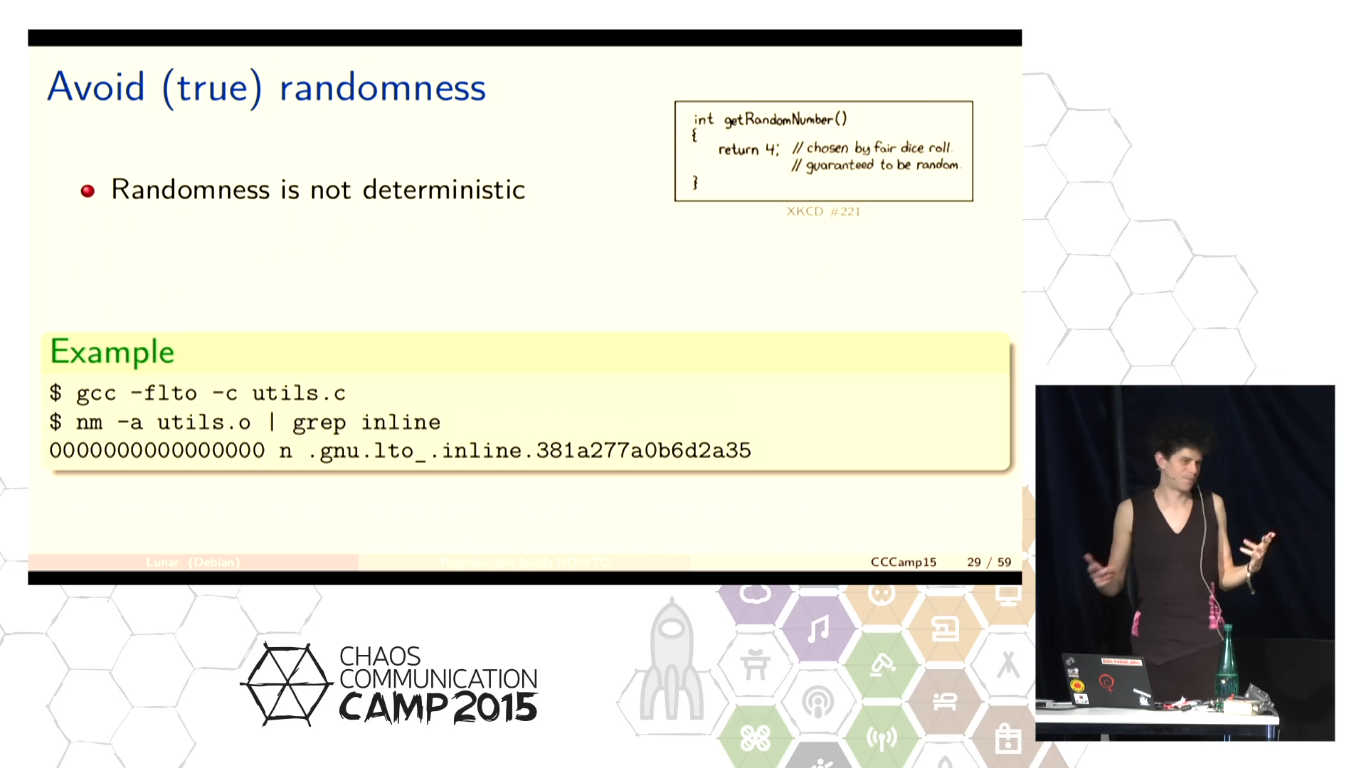
\includegraphics[width=0.83\textwidth]{images/cccamp2015_lunar_random.png}
  };
 \end{tikzpicture}
 \end{itemize}
\end{frame}


\begin{frame}
 \frametitle{\texttt{SOURCE\_DATE\_EPOCH}}

 \begin{itemize}
  \item Build date (timestamps) usually not useful for the user
  \item \texttt{SOURCE\_DATE\_EPOCH} is defined as the last modification of
  the source, since the epoch (1970-01-01)
  \item can be used instead of current date
  \item can also be used for random seeds etc.
  \item in Debian, set from the latest \texttt{debian/changelog} entry
  \item can be set to the latest git commit too or the latest file
  modification date
 \end{itemize}
\end{frame}

\begin{frame}
 \frametitle{\texttt{SOURCE\_DATE\_EPOCH}}

 \begin{itemize}
  \item \texttt{SOURCE\_DATE\_EPOCH} spec available:
  \item \texttt{https://reproducible-builds.org/specs/}
  \item many upstreams support it already
  \item has been adopted by other distributions
  (NetBSD, FreeBSD, Arch Linux, Guix, …)
 \end{itemize}
\end{frame}


\begin{frame}
 \frametitle{tests.reproducible-builds.org}

 \begin{itemize}
  \item Continuously testing Debian \texttt{testing}, \texttt{unstable} and
  \texttt{experimental}
  \item Also testing: coreboot, OpenWrt, LEDE, NetBSD, FreeBSD,
  Arch Linux, Fedora and soon F-Droid and Guix too
  \item 230 jenkins jobs
  \item 7 \texttt{amd64} nodes, 120 cores and 300 GB ram
  \item 15 \texttt{armhf} nodes, 54 cores and 25 GB ram
  \item 42 scripts in Python and Bash, 282 lines of code in average
  \item 29 contributors for \texttt{jenkins.debian.net.git}
 \end{itemize}
\end{frame}


\begin{frame}[fragile]
 \frametitle{Variations (when testing Debian)}

 \begin{center}
  \begin{table}
   \resizebox{0.95\textwidth}{!}{%
    \begin{tabular}{l|ll}
\textbf{variation} & \textbf{first build} & \textbf{second build} \\
\hline
hostname & \texttt{jenkins} & \texttt{i-capture-the-hostname} \\
domainname & \texttt{debian.net} & \texttt{i-capture-the-domainname} \\
\texttt{env TZ} & \texttt{GMT+12} & \texttt{GMT-14} \\
\texttt{env LANG} & \texttt{C} & \texttt{fr\_CH.UTF-8} \\
\texttt{env LC\_ALL} & not set & \texttt{fr\_CH.UTF-8} \\
\texttt{env USER} & \texttt{pbuilder1} & \texttt{pbuilder2} \\
uid & \texttt{1111} & \texttt{2222} \\
gid & \texttt{1111} & \texttt{2222} \\
UTS namespace & shared with the host & \textit{modified using \texttt{/usr/bin/unshare --uts}} \\
kernel version & Linux 3.16 or 4.X & on amd64 always varied, on armhf
sometimes \\
umask & 0022 & 0002 \\
CPU type & \multicolumn{2}{l}{same for both builds on amd64 \textit{(work in progress)}} \\
 & on armhf varied a bit & \\
filesystem & \multicolumn{2}{l}{same for both builds on amd64: (\texttt{tmpfs}), on armhf \texttt{ext3/4}} \\
 & & \textit{(and we have} \texttt{disorderfs}\textit{, but the code is disabled)} \\
year, month, date & \multicolumn{2}{l}{on amd64: 398 days variation, on armhf not yet} \\
hour, minute & \multicolumn{2}{l}{hour is usually the same… usually, the minute differs… } \\
\textit{everything else} & \multicolumn{2}{l}{\textit{is likely the same…}}
    \end{tabular}
   }
  \end{table}
 \end{center}
\end{frame}


\placelogofalse

{
\usebackgroundtemplate{%
 \begin{tikzpicture}[remember picture,overlay]%
  \node[shift={(-0.1\paperwidth, 0.15\paperheight)},at=(current page.south east)] {
    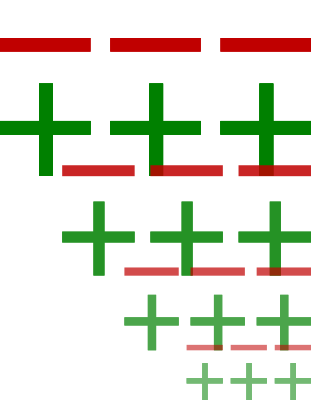
\includegraphics[width=0.2\paperwidth]{images/diffoscope_logo.png}
  };
 \end{tikzpicture}%
}

\begin{frame}{diffoscope}
 \frametitle{Debugging problems: \texttt{https://try.diffoscope.org}}

 \begin{itemize}
  \item Examines differences \textbf{in depth}.
  \item Outputs HTML or plain text with human readable differences.
  \item Recursively unpacks archives, uncompresses PDFs, disassembles
  binaries, unpacks Gettext files, …
  \item Easy to extend to new file formats.
  \item Falls back to binary comparison.
  \item Available from \texttt{git}, PyPI, Debian, \\
   Arch Linux, Guix, Homebrew. Works on BSD.
  \item Maintainers in other distros wanted.
  \item \url{https://diffoscope.org/}
 \end{itemize}
\end{frame}


\begin{frame}
 \frametitle{\texttt{diffoscope} example (HTML output)}
 \begin{tikzpicture}[remember picture]
  \node[at=(current page.center)] {
   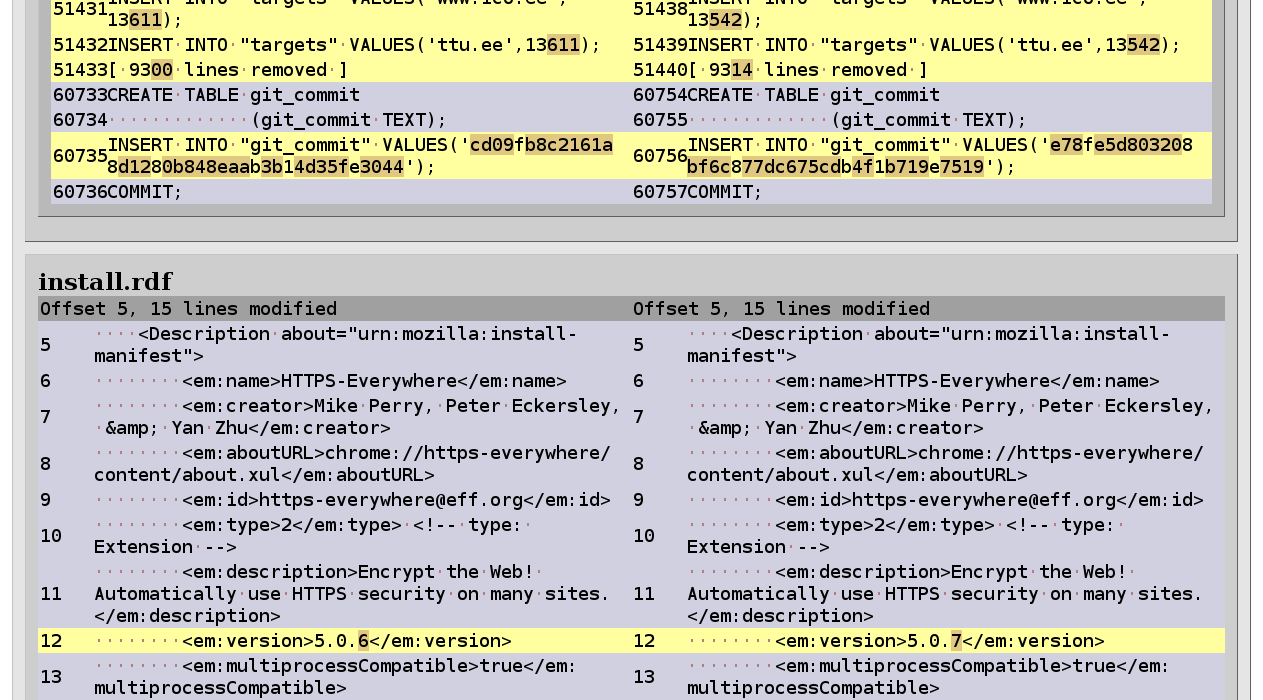
\includegraphics[width=0.9\paperwidth]{images/diffoscope_example_html.png}
  };
 \end{tikzpicture}
\end{frame}


\begin{frame}
 \frametitle{\texttt{diffoscope} is "just" for debugging}

 \begin{itemize}
  \item Reminder: \texttt{diffoscope} is for \textbf{debugging}
  \item "reproducible" according to our definition means: \textbf{bit by bit
  identical}. So the tools for testing whether something is reproducible are
  either \texttt{diff} or \texttt{sha256sum}!
 \end{itemize}
\end{frame}

}

\placelogotrue


\section{Status Debian}

\begin{frame}
 \frametitle{Progress in Debian \texttt{unstable}}
 \begin{tikzpicture}[remember picture]
  \node[shift={(-0.5\paperwidth, \paperheight)},at=(current page.south east)] {
    \includegraphics[height=0.65\paperheight]{images/stats_pkg_state.png}
  };
 \end{tikzpicture}
 \begin{center}
  \footnotesize{20,079 (85\%) out of 23,595 source packages are reproducible \\
    in our test framework}
  \vfill
 \end{center}
\end{frame}


\begin{frame}
 \frametitle{Debian packages on tests.reproducible-builds.org}
 \begin{itemize}
  \item \url{https://reproducible.debian.net/$src}
  \item 32 package sets 
 \end{itemize}
\end{frame}

\begin{frame}
 \frametitle{Notes and issues on tests.reproducible-builds.org}

 \begin{itemize}
  \item 179 categorised distinct issues
  \item 3,792 notes
  \item 2549 unreproducible packages in \texttt{sid}, but only 139 without a note
  \item 728 packages failing to build, but only 74 without a note
  \item maintained in \texttt{notes.git}
  \item currently Debian only, but cross distro notes are planned
 \end{itemize}
\end{frame}



\begin{frame}
 \frametitle{Progress in the Debian bug tracker}
 \begin{tikzpicture}[remember picture]
  \node[shift={(-0.5\paperwidth, \paperheight)},at=(current page.south east)] {
    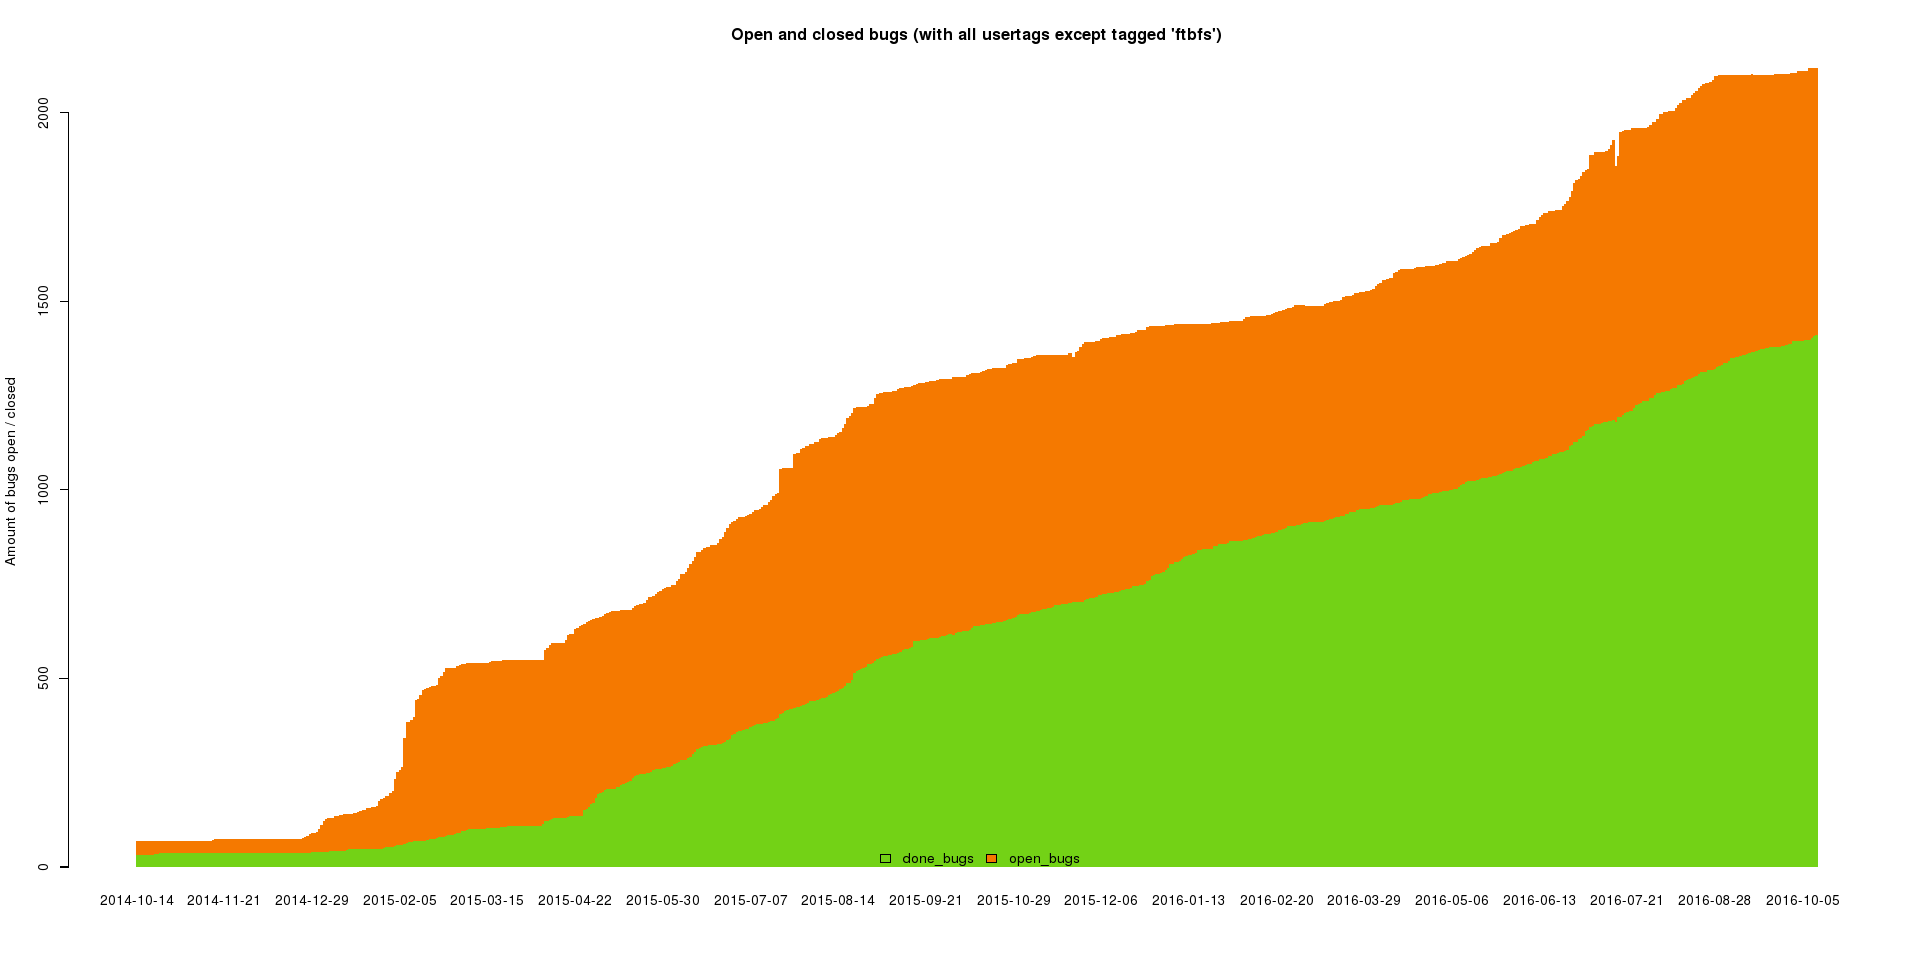
\includegraphics[height=0.65\paperheight]{images/stats_bugs_sin_ftbfs_state.png}
  };
 \end{tikzpicture}
 \begin{center}
  \footnotesize{As a rule, we file bugs with patches. \\
  There are very few exceptions.}
  \vfill
 \end{center}
\end{frame}


\begin{frame}
 \frametitle{Tell the world \& collaborate}

 \begin{itemize}
  \item "We don't care about Debian (only), we care about free and open
   source software."
  \item<2-4> Weekly reports since May 2015
  \item<3-4> First Reproducible World Summit in December 2015 (Athens, Greece)
   \begin{itemize}
    \item<3-4> 40 people from 16 projects
    \item<3-4> \texttt{reproducible.debian.net} has become \texttt{tests.reproducible-builds.org}
   \end{itemize}
    \item<4> Second Reproducible World Summit in December 2016 in Berlin
   \begin{itemize}
    \item<4> Talk to h01ger if you want to attend.
   \end{itemize}
 \end{itemize}
\end{frame}

\begin{frame}
 \frametitle{Reminder / Summary}
 \begin{itemize}
  \item This is just a proof-of-concept, Debian is not 85\% reproducible
  \item Debian "unstable" this summer?!!
  \item<2-3> I hope that Debian 9, "stretch", will be partially reproducible
  in a meaningful way, in 2017.
  \item<2-3> Will Debian 10, "buster", be 100\% reproducible?
  \item<3> What's beyond (rebuilding, \texttt{.buildinfo} file handling, user
  tools) mostly still needs \it{design} and code
 \end{itemize}
\end{frame}

\begin{frame}[plain]
 \begin{tikzpicture}[remember picture,overlay]
  \node[at=(current page.center)] {
    
\includegraphics[height=1.25\paperheight]{images/wholeworld.jpg}
    % Credits to Kevin ‘Chuise’ Jackson
    % http://dumhi.com/about
  };
 \end{tikzpicture}
\end{frame}


\section{Status Non-Debian World}

\placelogofalse



\begin{frame}
 \frametitle{OpenWrt and LEDE}
 \begin{itemize}
  \item \texttt{https://tests.r-b.org/openwrt}
  \item \texttt{https://tests.r-b.org/lede}
  \item maintained by lynxis, deki and h01ger
  \item 1000 packages build, 1/12 (OpenWrt/LEDE) images build
  \item packages look good, but not all variations tested yet
  \item images not yet.
 \end{itemize}
\end{frame}

\begin{frame}
 \frametitle{OpenWrt and LEDE cont.}
 \begin{itemize}
  \item collaboration: \texttt{notes.git} shall get multi-arch support
  \item more variations to be tested
 \end{itemize}
\end{frame}

\begin{frame}
 \frametitle{Skipped stati}
 \begin{itemize}
  \item \texttt{https://tests.r-b.org/coreboot}
  \item \texttt{https://tests.r-b.org/netbsd}
  \item \texttt{https://tests.r-b.org/freebsd}
  \item paused: \texttt{https://tests.r-b.org/archlinux}
  \item paused: \texttt{https://tests.r-b.org/fedora}
  \item not yet: \texttt{https://tests.r-b.org/f-droid}
 \end{itemize}
\end{frame}


\begin{frame}
 \frametitle{Unmentioned, with known activities}
 \begin{itemize}
\item Bitcoin (2011)
\item Tor (2013)
    \item NixOS
    \item Qubes, Tails
\item    few commercial, propietary Software
\item ?
 \end{itemize}
\end{frame}


\placelogotrue

\section{Future work}

\begin{frame}
 \frametitle{Rebuilders and sharing signed checksums}
 \begin{itemize}
  \item Almost no work has been done here yet. We are just at the first step:
  being able to rebuild reproducibly…
  \item Different projects, different solutions?
 \end{itemize}
\end{frame}

\begin{frame}
 \frametitle{Rebuilders and sharing signed checksums, cont.}
 \begin{itemize}
  \item Individuelly signed checksums (think web of trust) could work in the
  Debian case (we have a gpg web of trust), but IMO won't scale.
  \item { Another idea: rebuilders, run by large organisations
  (ACLU, CCC, CERN, Deutsche Bank, EDF, EON, Greenpeace, NASA, NSA, XYZ).}
  \item Fedora rebuilds Debian, Debian rebuilds OpenSUSE, OpenSUSE rebuilds
  NetBSD, etc…
  \item Big customers could just rebuild everything themselves.
 \end{itemize}
\end{frame}


\begin{frame}
 \frametitle{Integration in user tools}
 \begin{itemize}
  \item "Do you really want to install this unreproducible software (y/N)"
  \item<2-3> "Do you want to build those packages which unconfirmed checksums,
  before installing? (Y/n)"
  \item<3>{ "How many signed checksums do you require to call a package
  'reproducible'?" - and whom do you trust?}
 \end{itemize}
\end{frame}


\section{Getting involved}

\begin{frame}
 \frametitle{As a software developer}
 \begin{itemize}
  \item Stop using build dates
  \item Use \texttt{SOURCE\_DATE\_EPOCH} instead
  \item See \url{https://reproducible-builds.org/specs/}
 \end{itemize}
\end{frame}

\begin{frame}
 \frametitle{Getting involved - learning by doing}

 \begin{itemize}
  \item Test for yourself:
   \begin{itemize}
    \item Build something twice, run diffoscope on the results
    \begin{itemize}
     \item For better results use our “reproducible” repository, \texttt{pbuilder} and a custom config
    \end{itemize}
   \end{itemize}
  \item Docs on the web: \\
    \small{\url{https://reproducible-builds.org/docs/}} \\
    \small{\url{https://wiki.debian.org/ReproducibleBuilds/ExperimentalToolchain}}
  \item Ask for help on \texttt{\#reproducible-builds} or on mailing list
 \end{itemize}
\end{frame}


\begin{frame}
 \frametitle{Form your reproducible builds team!}

 \begin{itemize}
  \item Why?
   \begin{itemize}
    \item Every distribution should be reproducible!
    \item Learn something new everyday
    \item Change the (software) world!
    \item \texttt{https://tests.reproducible-builds.org/openwrt} needs \textbf{your} help
    \item \texttt{https://tests.reproducible-builds.org/lede} needs \textbf{your} help
   \end{itemize}
  \item How to get started?
   \begin{itemize}
    \item Talk to lynsis or h01ger here or talk to us on IRC or via mail.
    \item RTFM, there is lots of documentation
    \item Experiment - learning by doing
    \item Use+debug existing patches to \texttt{rpm-build}
   \end{itemize}
 \end{itemize}
\end{frame}

\section{Questions, comments, ideas?}


\begin{frame}
 \frametitle{Questions, comments, ideas?}

 \begin{itemize}
  \item \url{https://reproducible-builds.org/}
  \item \texttt{\#reproducible-builds} on \texttt{irc.OFTC.net}
  \item \url{https://lists.reproducible-builds.org}
  \item \url{https://twitter.com/ReproBuild}
  \item Mike and Seth's talk from 31c3 about motivations
  \item Lunar's talk about fixing reproducible issues from CCCamp 15
  \item h01ger's talk "the Reproducible builds ecosystem" from FOSDEM 16
  \end{itemize}
\end{frame}


\begin{frame}
 \frametitle{Thanks to…! …and thank \textbf{you}, too!}

 \begin{itemize}
  \item
    \only<1>{Debian “Reproducible Builds” team \\
        {\small (you are just \textbf{so} awesome!)}}
    \only<2>{All “Reproducible Builds” teams \\
        {\small (you are just \textbf{so} awesome!)}}
  \item Linux Foundation and the Core Infrastructure Initiative
  \item OpenWrt Summit
\end{itemize}

 \begin{center}
  
\includegraphics[height=0.1\paperheight]{images/linux_foundation_logo.png}
  \hspace{0.1\paperwidth}
  
\includegraphics[height=0.1\paperheight]{images/cii_logo.png}
 \end{center}

 \vfill
 \begin{center}
  \resizebox{0.9\textwidth}{!}{%
   \begin{tabular}{rl}
    \texttt{holger@debian.org} & \texttt{B8BF 5413 7B09 D35C F026} \\
                               & \texttt{FE9D 091A B856 069A AA1C} \\
    \texttt{lynxis@fe80.eu} & \texttt{390D CF78 8BF9 AA50 4F8F} \\
                               & \texttt{F1E2 C29E 9DA6 A0DF 8604}
\end{tabular}
  }
 \end{center}
\end{frame}

\begin{frame}{}
\begin{textblock}{12}(2, 6)
    \tiny{
      Copyright \copyright{} 2014--2016 \\
         Holger Levsen \texttt{holger@layer-acht.org} and others.\\[3.0mm]
      Copyright of images included in this document are held by
      their respective owners.
      \\[3.0mm]
      This work is licensed under the \alert{Creative Commons
        Attribution-Share Alike 3.0} License.  To view a copy of this
      license, visit
      \url{http://creativecommons.org/licenses/by-sa/3.0/} or send a
      letter to Creative Commons, 171 Second Street, Suite 300, San
      Francisco, California, 94105, USA.
      \\[2.0mm]
      % Give a link to the 'Transparent Copy', as per Section 3 of the GFDL.
      The source of this document is available from
      \url{https://anonscm.debian.org/git/reproducible/presentations.git}.
    }
  \end{textblock}
\end{frame}

\end{document}
